\documentclass{llncs}  

\usepackage{url}
\usepackage{algorithm2e}
\usepackage{amsmath}
\usepackage{amssymb}
\usepackage{etoolbox}
\usepackage{multirow}     
\usepackage[usenames,dvipsnames]{color}
\usepackage{tikz}
\usetikzlibrary{arrows,calc}
\usepackage{caption}
\usepackage{subcaption}
\usepackage{varwidth}
\captionsetup{compatibility=false}
\usepackage{listings}
\lstset{
  morekeywords={define,end,if,then,else,return,assume,assert},
  basicstyle=\ttfamily,
  keywordstyle=\underline,
  numbers=left,
  frame=l
}
\usepackage{bussproofs}

\newcommand{\smallnode}[1]{\begin{varwidth}{0.4cm}\scalebox{0.9}{\hspace{-0.2cm}#1}\end{varwidth}}
\newcommand{\todo}[1]{\textcolor{red}{{#1}}}
\newcommand{\hide}[1]{}
\newcommand{\fun}[1]{\mathtt{{#1}}}
\newcommand{\TT}{\mathtt{true}}

 
%\newcommand{\longversion}{}
\ifdef{\longversion}{
\newcommand{\whenlongversion}[1]{#1}
}{
\newcommand{\whenlongversion}[1]{}
}

\newcommand{\ox}{\textbf{x}}
\newcommand{\ou}{\textbf{u}}
\newcommand{\ov}{\textbf{v}}
\newcommand{\oE}{\textbf{E}}
\newcommand{\assert}[1]{(\!| {#1} |\!)}

\title{Verifying Recursive Programs using Intraprocedural Analyzers}
\author{Yu-Fang~Chen\inst{1} \and Chiao~Hsieh\inst{1,2} \and 
  Ming-Hsien~Tsai\inst{1} \and Bow-Yaw~Wang\inst{1} \and Farn~Wang\inst{2}}

\institute{
Institute of Information Science, 
Academia Sinica, Taiwan
\and
Graduate Institute of Electrical Engineering,
National Taiwan University, Taiwan
}

\pagestyle{plain}
\sloppy

\begin{document}
\maketitle

\begin{abstract}

Recursion can complicate program analysis significantly. 
Some program analyzers simply ignore recursion or even refuse
to check 
recursive programs. In this paper, we propose an algorithm that uses
a recursion-free program analyzer as a black box to check recursive
programs. With extended program constructs for assumptions,
assertions, and nondeterminsitic values, our algorithm computes
function summaries from inductive invariants computed by the
underlying program analyzer. Such function summaries enable our
algorithm to check recursive programs. We implement a prototype using
the recursion-free program analyzer \textsc{CPAChecker}, and compare
with other program analyzers on the benchmarks in the 2014 Competition
on Software Verification.

\end{abstract}

\section{Introduction}
\label{section:introduction}

Program verification is a grand challenge with significant impact in computer science.
Its main difficulty is in great part due to common program features such as concurrent execution, \hide{of threads,} pointers, \hide{with unbounded heap size,} recursive function calls, \hide{with recursions,} and unbounded basic data types~\cite{ClarkeJS05}. Subsequently, it is extremely complicated to develop a verification algorithm that handles all features. Researches on program verification typically address some of these features and simplify others. Verification tools however are required to support as many features as possible. Since implementation becomes increasingly unmanageable with additional features, incorporating algorithms for all features in verification tools can be a nightmare for developers.

One way to address the implementation problem is by reduction. If verifying a new feature can be transformed to existing features, development efforts can be significantly reduced.
In this paper, we propose an algorithm to extend intraprocedure (recursive-free) program analyzers to verify recursive programs. Such analyzers supply an \emph{inductive invariant} when a program is verified to be correct, and support program constructs such as assumptions, assertions, and nondeterministic values. Our algorithm transforms any recursive program into non-recursive ones, and invokes an intraprocedure program analyzer to verify properties about the generated non-recursive programs. The verification results allow us to infer properties on the given recursive program.

Our algorithm proceeds by iterations. In each iteration, it transforms the recursive program into a non-recursive program that \emph{under-approximates} the behaviors of the original and sends the under-approximation to an intraprocedure program analyzer. If the analyzer verifies the under-approximation, purported \emph{function summaries} for recursive functions are computed. Our algorithm transforms the original recursive program into more non-recursive programs with purported function summaries. It then checks if purported function summaries are correct by sending these non-recursive programs to the analyzer.

The advantages of the proposed algorithm is clear: it requires only very few and standard functions provided by the underlying verifiers and is compatible with most existing intraprocedure analyzers. We implemented a prototype system using \textsc{CPAChecker}~\cite{BeyerK11} as the underlying program analyzer and compare
with other program analyzers that are specialized for recursive program verification on the benchmarks in the 2014 Competition on Software Verification~\cite{svcomp14}.
The comparison result is very promising: the prototype is comparable with those specialized analyzers. Notice that in order to simplify the implementation effort, we turned off important optimizations such as adjust block encoding provided in \textsc{CPAChecker}, the performance of the prototype can be even better with those optimizations turned on. 

\subsection*{Related Works}
Inter-Procedure analyzers
Whale~\cite{AlbarghouthiGC12},
Ultimate Automizer~\cite{HeizmannCDEHLNSP13}
Ultimiate Kojak~\cite{Kojak}
RHS~\cite{RepsHS95} (say we can achieve the same by ...)
SLAM~\cite{BallR01}

Difference compared with Whale

In general, Whale tries to extend Lazy Abstraction to verify interprocedual program.
It mainly constructs an iARG with path conditions that can encode function calls and check for reachability of bug.
Also it introduces an extended covering relation over summaries of function calls to deal with recursion.
Our work, however, uses bounded times of unwinding to construct paths across functions,
and we find reasonable summaries for recursive functions when proving safety of program.

For guessing summaries, both Whale and our work use under-approximation of function calls.
In Whale, the under-approximation of a function call is constructed through exploring paths without function call in the called function.
In our work, the function call is unwinded and transformed, and the exploration is achieved by the program analyzer we used.
With our method, we can create more precise under-approximation by unwinding more times before tranforming.

For proving summaries, Whale and our work apply the Hoare rule of recursion. Whale defines the covering relation between summaries upon Hoare rule of consequence for proving. Our work, in other way, directly proves by the used program analyzer.

Intra-procedure analyzers
UFO~\cite{AlbarghouthiLGC12}
Blast~\cite{BeyerHJM07}





\section{Preliminaries}
\label{section:preliminaries}


Let $\mathtt{Vars}$ denote the set of \emph{program variables} and
$\mathtt{Vars}' = \{ \ox' : \ox \in \mathtt{Vars} \}$.
We consider a variant of the WHILE language~\cite{}:
\begin{equation*}
  \begin{array}{rccll}
    \mathtt{Expression} & \ni E & ::= &
    \mathtt{x} & \mathtt{x} \in \mathtt{Vars}\\
    & & \mid &
    \mathtt{false}\ \mid\ \mathtt{true}\ \mid\ 
    \mathtt{0}\ \mid\ \mathtt{1}\ \mid\ \ldots\hspace{.06\textwidth} &
    \textmd{constant}\\
    & & \mid &
    \mathtt{nondet} & \textmd{nodeterministic value}\\
    & & \mid &
    \mathtt{f}(E, E, \ldots, E) &
    \textmd{function invocation}\\
    & & \mid &
    E \odot E  & \odot \in \{ +, -, =, >, \mathtt{and}, \mathtt{or} \}\\
    & & \mid & \mathtt{not}\ E\\
    \mathtt{Command} & \ni C & ::= &
    \mathtt{x}, \mathtt{x}, \ldots, \mathtt{x} := 
    E, E, \ldots, E & \textmd{assignment}\\
    & & \mid &
    C\mathtt{;}\ C &
    \textmd{sequential composition}\\
    & & \mid &
    \mathtt{return}\ E, E, \ldots, E & \textmd{function return}\\
    & & \mid &
    \mathtt{assume}\ E & \textmd{assumption}\\
    & & \mid &
    \mathtt{assert}\ E & \textmd{assertion}
  \end{array}
\end{equation*}
The $\mathtt{nondet}$ expression evaluates to a type-safe
nondeterministic value.
Note that simultaneous assignments are allowed in our language. To
execute a simultaneous assignment, all expressions on the right hand
side are first evaluated and then assign to respective variables. 
The $\mathtt{return}$ command accepts several expressions as arguments.
Together with simultaneous assignments, functions can have several
return values. 
The assumption command excludes all computation not satisfying the given
expression. The assert command terminates computation
abnormally if the given expression is not satisfied. For
instance, the following command always terminates normally:
\begin{equation*}
  \mathtt{assume\ false};\ \ \mathtt{assert\ false}
\end{equation*}
\todo{no computation means terminate normally?}




A function is represented as a \emph{control flow graph} $G = \langle
V, E,\textmd{cmd} \rangle$ where the nodes in $V$ are \emph{program locations}, and
each edge $(\ell, \ell')$ in $E \subseteq V \times V$ is labeled by a
command denoted by $\textmd{cmd} (\ell, \ell')$. We
assume that the program locations $\ell_s$ and $\ell_e$ denote the
entry and exit of each function. Moreover, the special
$\mathtt{main()}$ function specifies where a program starts.
We use $G_f=\langle
V_f, E_f,\textmd{cmd}_f \rangle$ to denotes the CFG corresponds to a the function $\mathtt{f}$.
Figure~\ref{figure:mccarthy91} shows control flow graphs for the
McCarthy 91 program. The $\mathtt{main()}$ function assumes the
variable $\mathtt{n}$ is non-negative. It then checks if the return
value of $\mathtt{mc91(n)}$ is no less than 90
(Figure~\ref{figure:mccarthy91:main}). The $\mathtt{mc91(m)}$ function
branches on whether the variable $\mathtt{m}$ is greater than 100. If
so, the return value $\mathtt{ret^{mc91}_0}$ is set to $\mathtt{m} -
10$. Otherwise, 
$\mathtt{mc91(m)}$ assigns the return value of $\mathtt{mc91(m + 11)}$
to $\mathtt{s}$, and updates $\mathtt{ret^{mc91}_0}$ by calling
$\mathtt{mc91(s)}$ recursively
(Figure~\ref{figure:mccarthy91:mc91}). Observe that the 
$\mathtt{assume}$ command models a conditional branch in the
figure. Loops can be modeled similarly.

\begin{figure}
  \centering
  \begin{subfigure}[b]{.3\textwidth}
    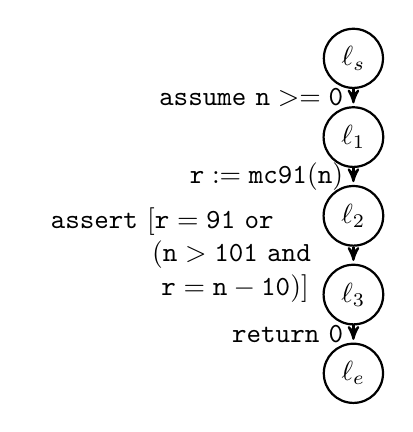
\begin{tikzpicture}[->,>=stealth',shorten >=1pt,auto,node
      distance=2cm,thick,node/.style={circle,draw}]
      \node[node] (0) at (0, 0) {$\ell_s$}; %[label=above:$\mathtt{main()}$]
      \node[node] (1) at (0, -1) {$\ell_1$};
      \node[node] (2) at (0, -2) {$\ell_2$};
      \node[node] (3) at (0, -3) {$\ell_3$};
      \node[node] (4) at (0, -4) {$\ell_e$};

      \path
        (0) edge 
            node [left] {$\mathtt{assume\ n >= 0}$} (1)
        (1) edge 
            node [left] {$\mathtt{r := mc91(n)}$} (2)
        (2) edge 
            node [left] {$
              \begin{array}{l}
                \mathtt{assert\ {[}r = 91\ or}\\
                \mathtt{\ \ \ \ \ \ \ \ \ \ \ (n > 101\ and\ \ }\\
                \mathtt{\ \ \ \ \ \ \ \ \ \ \ \ r = n - 10){]}}
              \end{array}$} (3) 
        (3) edge 
            node [left] {$\mathtt{return\ 0}$} (4);
    \end{tikzpicture}
    \caption{$\mathtt{main()}$}
    \label{figure:mccarthy91:main}
  \end{subfigure}
  ~
  \begin{subfigure}[b]{.6\textwidth}
    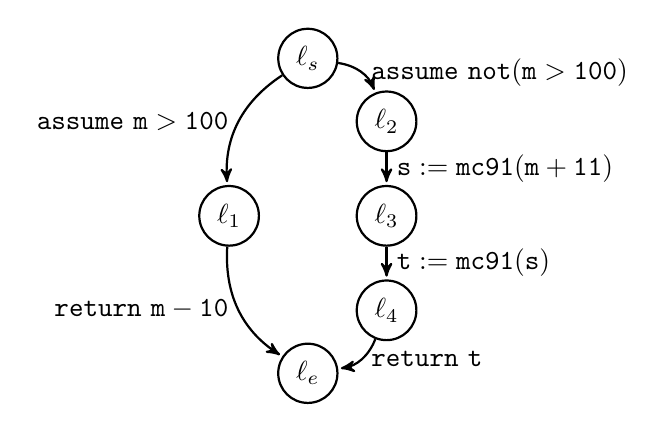
\begin{tikzpicture}[->,>=stealth',shorten >=1pt,auto,node
      distance=2cm,thick,node/.style={circle,draw}]
      \node[node] (0) at ( 0,  0) {$\ell_s$}; %[label=above:$\mathtt{mc91(n)}$]
      \node[node] (1) at (-1, -2) {$\ell_1$};
      \node[node] (2) at ( 1, -0.8) {$\ell_2$};
      \node[node] (3) at ( 1, -2) {$\ell_3$};
      \node[node] (4) at ( 1, -3.2) {$\ell_4$};
      \node[node] (5) at ( 0, -4) {$\ell_e$};

      \path
        (0) edge [bend right=30]
            node [left] {$\mathtt{assume\ m > 100}$} (1)
            edge [bend left=30]
            node [right] {$\mathtt{assume\ not(m > 100)}$} (2)
        (1) edge [bend right=30]
            node [left] {$\mathtt{return\ m - 10}$} (5)
        (2) edge 
            node [right] {$\mathtt{s := mc91(m + 11)}$} (3)
        (3) edge 
            node [right] {$\mathtt{t := mc91(s)}$} (4)
        (4) edge [bend left=30]
            node [right] {$\mathtt{return\ t}$} (5);
    \end{tikzpicture}
    \caption{$\mathtt{mc91(m)}$}
    \label{figure:mccarthy91:mc91}
  \end{subfigure}
  \caption{McCarthy 91}
  \label{figure:mccarthy91}
\end{figure}

\todo{definitions of accessible variables, program states}
Let $G = \langle V, E ,\textmd{cmd}\rangle$ be a control flow graph.
An \emph{inductive invariant} $\Pi (G, I_0) = \{ I_\ell : \ell \in V
\}$ for $G$ from $I_0$ is a set of first-order logic formulae such
that $I_{\ell_s} = I_0$, and for every $(\ell, \ell') \in E$
\begin{equation*}
I_{\ell} \wedge \tau_{\textmd{cmd}(\ell, \ell')} \implies I'_{\ell'}
\end{equation*}
where $I'$ is the formula obtained by replacing every $\ox \in
\mathtt{Vars}$ in $I$ with $\ox' \in \mathtt{Vars}'$, and
$\tau_{\textmd{cmd} (e)}$ specifies the semantics of the command
$\textmd{cmd} (e)$. An inductive invariant $\Pi (G, I_0)$ is an
over-approximation to the computation of $G$ from $I_0$. More
precisely, assume that the function $G$ starts from a state satisfying
$I_0$. For every program location $\ell$, $G$ must arrive in a state
satisfying $I_{\ell}$ when the computation reaches $\ell$. 

Let $G = \langle V, E,\textmd{cmd} \rangle$ be a control flow graph, and $P$, $Q$
are logic formulae. A \emph{Hoare triple} $\assert{P} G \assert{Q}$
specifies that the program $G$ will reach a program state satisfying
$Q$ provided that $G$ starts with a program state satisfying $P$ and
terminates. We use the standard proof rules for weak correctness with
two additional rules for the assumption and assertion commands:
\begin{center}
  \AxiomC{$P \wedge E \implies Q$}
  \LeftLabel{Assume}
  \UnaryInfC{$\assert{P} \mathtt{assume\ } E \assert{Q}$}
  \DisplayProof
  ~
  \AxiomC{$P \implies E$}
  \LeftLabel{Assert}
  \UnaryInfC{$\assert{P} \mathtt{assert\ } E \assert{Q}$}
  \DisplayProof
\end{center}
Observe
that an inductive invariant $\Pi (G, I_0)$ establishes 
$\assert{I_0} G \assert{I_{\ell_e}}$.

A \emph{program analyzer} accepts programs as inputs and
checks if all assertions (specified by the $\mathtt{assert}$ command)
are satisfied. One way to implement program analyzers is to compute
inductive invariants. 
\begin{proposition}
Let $G = \langle V, E,\textmd{cmd} \rangle$ be a control flow
graph and $\Pi (G, \mathtt{true})$ an inductive invariant for $G$ from
$\mathtt{true}$. If $\models I_{\ell} \implies B_{\ell}$ for every
edge $(\ell, \ell') \in E$ with $\textmd{cmd} (\ell, \ell') =
\mathtt{assert} (B_{\ell})$, then all assertions in $G$ are satisfied.
\end{proposition}
A program analyzer checks assertions by computing inductive invariants
is called an \emph{inductive} program analyzer. Note that an inductive
program analyzer need not give any information when an assertion fails. 
Indeed, most inductive program analyzers simply report false positives
when inductive invariants are too coarse. A \emph{program checker} is
a program analyzer that returns an error trace when an assertion
fails; an \emph{error trace} is a sequence of variable valuations from
the program entry to the failed assertion. Rather than reporting false
positives, program checkers have to return error traces to witness 
failed assertions. Producing error traces (especially for recursive
programs) complicates analysis algorithms. We hence consider a
subclass of program checker. A \emph{recursion-free
  inductive program checker} is a program checker that checks
recursion-free programs by computing inductive invariants, and reports
an error trace when an assertion fails. Several recursion-free
inductive program checkers are available such as \textsc{CPAChecker},
\textsc{Blast}, \textsc{UFO}, \textsc{}. Our goal is to check
recursive programs by using a recursion-free inductive program checker
as a black box. 


\section{Overview}
\label{section:overview}


Let \textsc{BasicChecker} denote a recursion-free inductive program
checker and $G = \langle V, E \rangle$ a control flow graph. Since
non-recursive functions can be replaced by their control flow graphs
after proper variable renaming, we assume that $G$ only contains the
$\mathtt{main()}$ and recursive functions. If $G$ does not contain
recursive functions, \textsc{BasicChecker} is able to check $G$ by
computing inductive invariants.

When $G$ contains recursive functions, we transform $G$ into a
recursion-free program $\underline{G}$. The program $\underline{G}$
under-approximates the computation of $G$. That is, every computation
of $\underline{G}$ is also a computation of $G$. If
\textsc{BasicChecker} finds an error trace in $\underline{G}$, our
algorithm terminates and reports the error trace. Otherwise,
\textsc{BasicChecker} has computed an inductive invariant for the
recursive-free under-approximation $\underline{G}$. Our algorithm
updates function summaries of $G$ from the inductive invariant of
$\underline{G}$. It then checks if every function summary
over-approximations the computation of the corresponding function. If
so, the algorithm terminates and reports that all assertions in $G$
are satisified. If a function summary does not over-approximate the
computation, our algorithm unwind the recursive function and
reiterates~(Algorithm~\ref{algorithm:overview}).

\begin{algorithm}
  \KwIn{$G = \langle V, E \rangle$ : a control flow graph}
  $k \leftarrow 0$\;
  $G_0 \leftarrow G$\;
  \lForEach{function $\mathtt{f}$ in $G$}
  {
    $S[\mathtt{f}] \leftarrow \mathtt{true}$\;
  }
  \Repeat{$\textmd{complete?}$}
  {
    \Switch{\textsc{BasicChecker} ($\underline{G}_k$)}
    {
      \lCase{$\mathit{Pass(\Pi (\underline{G}_k, I_0))}$:}
      {    
        UpdateSummary ($G$, $S$, $\Pi (\underline{G}_k, I_0)$)\;
      }
      \lCase{$\mathit{ErrorTrace} (\tau)$:}
      {
        \Return $\mathit{ErrorTrace} (\tau)$\;
      }
    }
    $\textmd{complete?} \leftarrow \top$\;
    \ForEach{function $\mathtt{f}$ in $G$}
    {
      \lIf {\textsc{BasicChecker} ($\overline{G}_{\mathtt{f}}$) =
        $\mathit{ErrorTrace}\ \_$}
      {
        $\textmd{complete?} \leftarrow \bot$\;
      }
    }
    $G_{k+1} \leftarrow $ unwind $G_k$\;
    $k \leftarrow k + 1$\;
  }
  \caption{Overview}
  \label{algorithm:overview}
\end{algorithm}

To see how to under approximate computation, consider a control flow
graph $G_k$ with recursive functions $f_0 (\ox_0), f_1 (\ox_1),
\ldots, f_m (\ox_m)$. The under-approximation $\underline{G}_k$ is
obtained by substituting the command $\mathtt{assume\ false}$ for
every command with recursive function calls
(Figure~\ref{figure:under-mccarthy91}). The substitution
effectively blocks all recursive invocations. Any computation of
$\underline{G}_k$ hence is also a computation of $G_k$. Note that
$\underline{G}_k$ is recursion-free. \textsc{BasicChecker} is able to
check the under-approximation $\underline{G}_k$.

\begin{figure}
  \centering
  \begin{subfigure}[b]{.3\textwidth}
    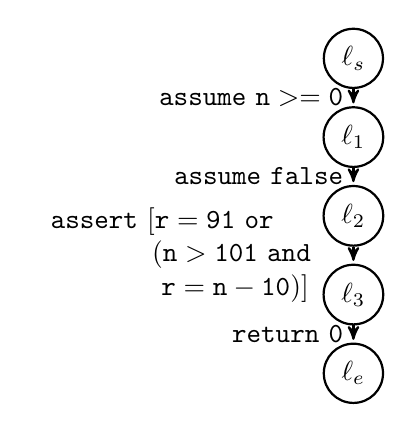
\begin{tikzpicture}[->,>=stealth',shorten >=1pt,auto,node
      distance=2cm,thick,node/.style={circle,draw}]
      \node[node] (0) at (0, 0) {$\ell_s$}; %[label=above:$\mathtt{main()}$]
      \node[node] (1) at (0, -1) {$\ell_1$};
      \node[node] (2) at (0, -2) {$\ell_2$};
      \node[node] (3) at (0, -3) {$\ell_3$};
      \node[node] (4) at (0, -4) {$\ell_e$};

      \path
        (0) edge 
            node [left] {$\mathtt{assume\ n >= 0}$} (1)
        (1) edge 
            node [left] {$\mathtt{assume\ false}$} (2)
        (2) edge 
            node [left] {$
              \begin{array}{l}
                \mathtt{assert\ {[}r = 91\ or}\\
                \mathtt{\ \ \ \ \ \ \ \ \ \ \ (n > 101\ and\ \ }\\
                \mathtt{\ \ \ \ \ \ \ \ \ \ \ \ r = n - 10){]}}
              \end{array}$} (3) 
        (3) edge 
            node [left] {$\mathtt{return\ 0}$} (4);
    \end{tikzpicture}
    \caption{$\mathtt{\underline{main}()}$}
  \end{subfigure}
  ~
  \begin{subfigure}[b]{.6\textwidth}
    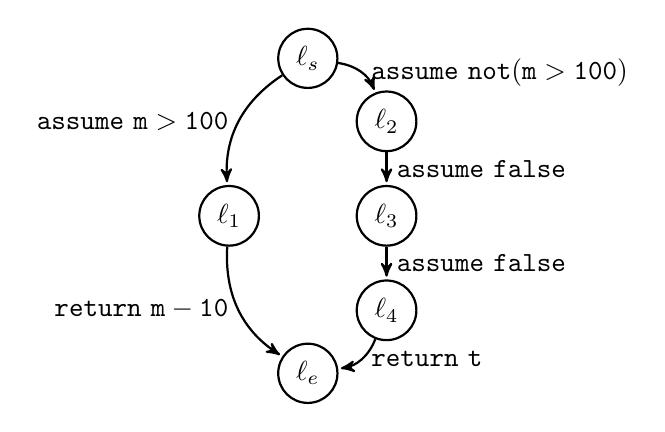
\begin{tikzpicture}[->,>=stealth',shorten >=1pt,auto,node
      distance=2cm,thick,node/.style={circle,draw}]
      \node[node] (0) at ( 0,  0) {$\ell_s$}; %[label=above:$\mathtt{mc91(n)}$]
      \node[node] (1) at (-1, -2) {$\ell_1$};
      \node[node] (2) at ( 1, -0.8) {$\ell_2$};
      \node[node] (3) at ( 1, -2) {$\ell_3$};
      \node[node] (4) at ( 1, -3.2) {$\ell_4$};
      \node[node] (5) at ( 0, -4) {$\ell_e$};

      \path
        (0) edge [bend right=30]
            node [left] {$\mathtt{assume\ m > 100}$} (1)
            edge [bend left=30]
            node [right] {$\mathtt{assume\ not(m > 100)}$} (2)
        (1) edge [bend right=30]
            node [left] {$\mathtt{return\ m - 10}$} (5)
        (2) edge 
            node [right] {$\mathtt{assume\ false}$} (3)
        (3) edge 
            node [right] {$\mathtt{assume\ false}$} (4)
        (4) edge [bend left=30]
            node [right] {$\mathtt{return\ t}$} (5);
    \end{tikzpicture}
    \caption{$\mathtt{\underline{mc91}(m)}$}
  \end{subfigure}
  \caption{Under Approximation of McCarthy 91}
  \label{figure:under-mccarthy91}
\end{figure}

When $\textsc{BasicChecker}$ does not find any error trace in the
under-approximation $\underline{G}_k$, it computes an inductive
invariant $\Pi (\underline{G}_k, I_0)$. Our algorithm then updates
summaries of functions in $G$. For each function $\mathtt{f}$ with
formal parameters $\mathtt{u_0}, \mathtt{u_1}, \ldots, \mathtt{u_l}$
and $h$ return values, a \emph{function summary} for $\mathtt{f}$ is a
first-order conjunctive formula which specifies the relation between
its formal parameters and return variables. The algorithm
$\textmd{UpdateSummary}$ updates function summaries $S$ by inspecting
the inductive invariant $\Pi (\underline{G}_k, I_0)$
(Section~\ref{subsection:property-proving}). 

After function summaries are updated, Algorithm~\ref{algorithm:overview} 
verifies whether function summaries correctly specify computation of
functions. The algorithm checks this by constructing a control flow
graph $\overline{G}_{\mathtt{f}}$ with additional assertions for each
function $\mathtt{f}$, and verifying $\overline{G}_{\mathtt{f}}$ with
\textsc{BasicChecker}. The control flow graph
$\overline{G}_{\mathtt{f}}$ is obtained by substituting function
summaries for function calls. In Algorithm~\ref{algorithm:overview},
$S[\mathtt{g}]$ contains the function summary for the function
$\mathtt{g}$.  
We transform $G_{\mathtt{f}}$ into $\overline{G}_{\mathtt{f}}$ by the
following three steps:
\begin{enumerate}
\item Replace every function call $\mathtt{x_1}, \mathtt{x_2}, \ldots,
  \mathtt{x_q} := \mathtt{g} (E_0, E_1, \ldots, E_p)$ in $G_{\mathtt{f}}$ by 
  \begin{equation*}
    \begin{array}{l}
      \mathtt{x_1}, \ldots, \mathtt{x_q} :=
      \mathtt{nondet}, \ldots, \mathtt{nondet};\\
      \mathtt{assume}\ 
      S[{\mathtt{g}}]\{\mathtt{u_0} \mapsto E_0, \ldots, 
      \mathtt{u_p} \mapsto E_p, \mathtt{ret^g_1} \mapsto \mathtt{x_1},
      \ldots, \mathtt{ret^g_q} \mapsto \mathtt{x_q}\}
    \end{array}
  \end{equation*}
  where $\mathtt{u_0}, \mathtt{u_1}, \ldots, \mathtt{u_p}$
  are the formal parameters of the function $\mathtt{g}$;
\item Replace every $\mathtt{return\ }F_1, F_2, \ldots, F_h$ command by
  \begin{equation*}
    \mathtt{ret^f_1}, \ldots, \mathtt{ret^f_h} := F_1, \ldots, F_h
  \end{equation*}
\item Add the command $\mathtt{assert\ }S[{\mathtt{f}}]$ at the end of
  $G_{\mathtt{f}}$. 
\end{enumerate}
Figure~\ref{figure:check-summary-mccarthy91} shows the control flow
graph $\overline{G}_{\mathtt{mc91}}$ with the function summary
$S[{\mathtt{mc91}}] = \mathtt{not (m \geq 0)}$. Observe that
$\overline{G}_{\mathtt{mc91}}$ is
recursion-free. \textsc{BasicChecker} is able to check the
over-approximation $\overline{G}_{\mathtt{mc91}}$. 

\begin{figure}
  \centering
    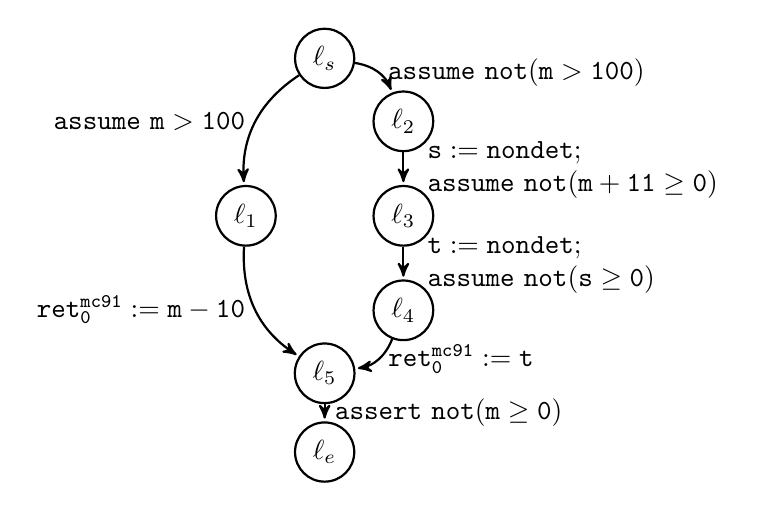
\begin{tikzpicture}[->,>=stealth',shorten >=1pt,auto,node
      distance=2cm,thick,node/.style={circle,draw}]
      \node[node] (s) at ( 0,  0) {$\ell_s$}; %[label=above:$\mathtt{mc91(n)}$]
      \node[node] (1) at (-1, -2) {$\ell_1$};
      \node[node] (2) at ( 1, -0.8) {$\ell_2$};
      \node[node] (3) at ( 1, -2) {$\ell_3$};
      \node[node] (4) at ( 1, -3.2) {$\ell_4$};
      \node[node] (5) at ( 0, -4) {$\ell_5$};
      \node[node] (e) at ( 0, -5) {$\ell_e$};

      \path
        (s) edge [bend right=30]
            node [left] {$\mathtt{assume\ m > 100}$} (1)
            edge [bend left=30]
            node [right] {$\mathtt{assume\ not(m > 100)}$} (2)
        (1) edge [bend right=30]
            node [left] {$\mathtt{ret^{mc91}_0 := m - 10}$} (5)
        (2) edge 
            node [right] {$
              \begin{array}{l}
              \mathtt{s := nondet;}\\
              \mathtt{assume\ not(m + 11 \geq 0)}
              \end{array}
              $} (3)
        (3) edge 
            node [right] {$
              \begin{array}{l}
              \mathtt{t := nondet;}\\
              \mathtt{assume\ not(s \geq 0)}
              \end{array}$} (4)
        (4) edge [bend left=30]
            node [right] {$\mathtt{ret^{mc91}_0 := t}$} (5)
        (5) edge 
            node [right] {$\mathtt{assert\ not(m \geq 0)}$} (e)
        ;
    \end{tikzpicture}
  \caption{Check Summary in McCarthy 91}
  \label{figure:check-summary-mccarthy91}
\end{figure}

In order to refine approximations, our algorithm unwinds recursive
functions as usual. More precisely, consider a recursive function
$\mathtt{f}$ with formal parameters $\mathtt{u_0}, \mathtt{u_1},
\ldots, \mathtt{u_l})$ and $h$ return values. Let $G_{\mathtt{f}}$ be
the control flow graph of $\mathtt{f}$ and $G_k$ a control flow graph
that invokes $\mathtt{f}$. To unwind $\mathtt{f}$ in $G_k$, 
we first construct a control flow graph $H_{\mathtt{f}}$ by 
replacing every $\mathtt{return}\ F_1, F_2, \ldots, F_h$ command in
$\mathtt{f}$ with the assignment $\mathtt{ret^f_1}, \mathtt{ret^f_2}, \ldots,
\mathtt{ret^f_h} := F_1, F_2, \ldots, F_h$. For each edge $(\ell,
\ell')$ labeled with the command $\mathtt{x_1}, \mathtt{x_2}, \ldots,
\mathtt{x_h} := \mathtt{f}(E_0, E_1, \ldots, E_l)$ in $G_k$, we remove
the edge $(\ell, \ell')$, make a fresh $H'_{\mathtt{f}}$ by
renaming every nodes and variables in $H_{\mathtt{f}}$, add an edge
from $\ell$ to the entry node of $H'_{\mathtt{f}}$ that assigns $E_0,
E_1, \ldots, E_l$ to fresh copies of formal parameters in
$H'_{\mathtt{f}}$, and another edge from the exit node to $\ell'$ that
assigns fresh copies of return variables to $\mathtt{x_1},
\mathtt{x_2}, \ldots, \mathtt{x_h}$. The control flow graph $G_{k+1}$
is obtained by unwinding every function calls in $G_k$. 
Figure~\ref{figure:unwind-mccarthy91} shows the control flow graph
$\mathtt{mc91_1(m)}$ by unwinding $\mathtt{mc91(m)}$. Note that the
unwinding graph $G_{k+1}$ still has recursive function calls. Its
under approximation $\underline{G}_{k+1}$ however is more informative
than $\underline{G}_k$.

\begin{figure}
  \centering
    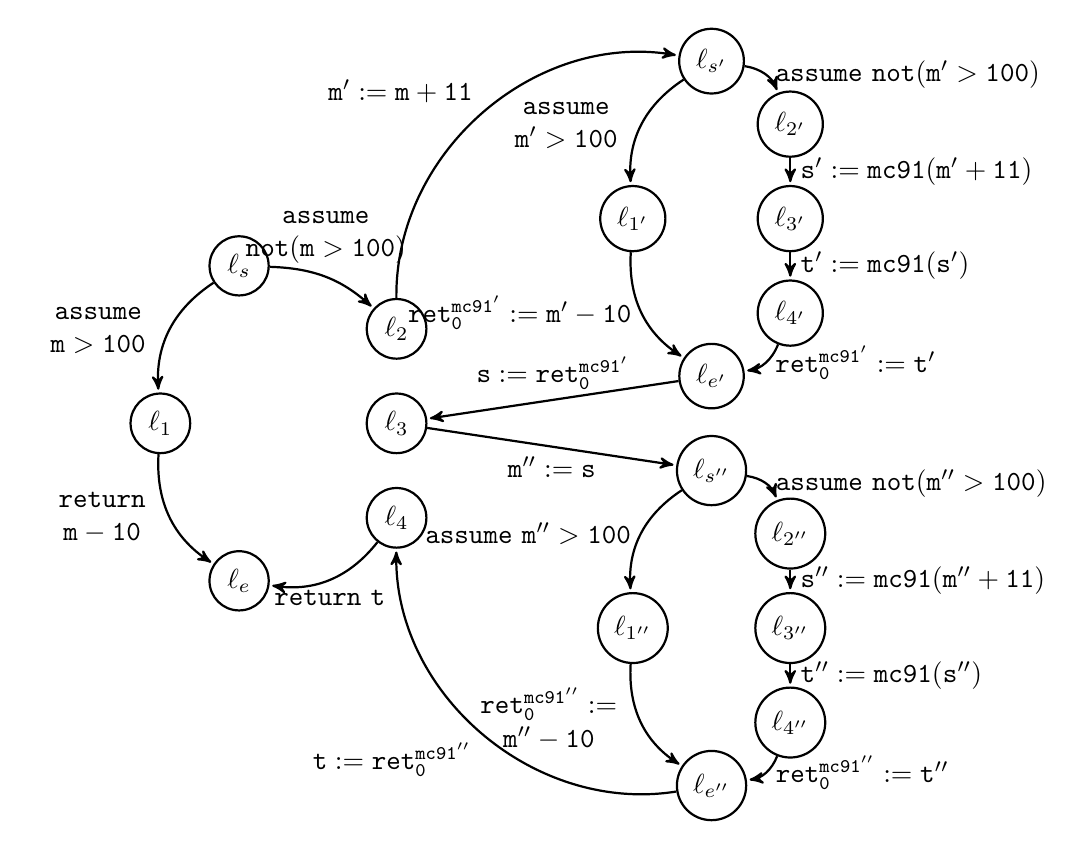
\begin{tikzpicture}[->,>=stealth',shorten >=1pt,auto,node
      distance=2cm,thick,node/.style={circle,draw}]
      \node[node] (s) at (-1,  0) {$\ell_s$};
      \node[node] (1) at (-2, -2) {$\ell_1$};
      \node[node] (2) at ( 1, -0.8) {$\ell_2$};
      \node[node] (3) at ( 1, -2) {$\ell_3$};
      \node[node] (4) at ( 1, -3.2) {$\ell_4$};
      \node[node] (e) at (-1, -4) {$\ell_e$};

      \node[node] (s') at ( 5,  2.6) {$\ell_{s'}$};
      \node[node] (1') at ( 4,  0.6) {$\ell_{1'}$};
      \node[node] (2') at ( 6,  1.8) {$\ell_{2'}$};
      \node[node] (3') at ( 6,  0.6) {$\ell_{3'}$};
      \node[node] (4') at ( 6, -0.6) {$\ell_{4'}$};
      \node[node] (e') at ( 5, -1.4) {$\ell_{e'}$};

      \node[node] (s'') at ( 5, -2.6) {$\ell_{s''}$};
      \node[node] (1'') at ( 4, -4.6) {$\ell_{1''}$};
      \node[node] (2'') at ( 6, -3.4) {$\ell_{2''}$};
      \node[node] (3'') at ( 6, -4.6) {$\ell_{3''}$};
      \node[node] (4'') at ( 6, -5.8) {$\ell_{4''}$};
      \node[node] (e'') at ( 5, -6.6) {$\ell_{e''}$};

      \path
        (s) edge [bend right=30]
            node [left] {$
              \begin{array}{c}
                \mathtt{assume}\\ 
                \mathtt{m > 100}                
              \end{array}$} (1)
            edge [bend left=20]
            node [above] {$
              \begin{array}{c}
                \mathtt{assume}\\
                \mathtt{not(m > 100)}
              \end{array}$} (2)
        (1) edge [bend right=30]
            node [left] {$
              \begin{array}{c}
                \mathtt{return}\\
                \mathtt{m - 10}
              \end{array}$} (e)
        (2) edge [bend left=50]
            node [above left] {$\mathtt{m' := m + 11}$} (s')
        (3) edge 
            node [below] {$\mathtt{m'' := s}$} (s'')
        (4) edge [bend left=30]
            node [below] {$\mathtt{return\ t}$} (e)

        (s') edge [bend right=30]
             node [left] {$
               \begin{array}{c}
                 \mathtt{assume}\\
                 \mathtt{m' > 100}
               \end{array}$} (1')
             edge [bend left=30]
             node [right] {$\mathtt{assume\ not(m' > 100)}$} (2')
        (1') edge [bend right=30]
             node [left] {$\mathtt{ret^{mc91'}_0 := m' - 10}$} (e')
        (2') edge 
             node [right] {$\mathtt{s' := mc91(m'+11)}$} (3')
        (3') edge 
             node [right] {$\mathtt{t' := mc91(s')}$} (4')
        (4') edge [bend left=30]
            node [right] {$\mathtt{ret^{mc91'}_0 := t'}$} (e')
        (e') edge 
             node [above] {$\mathtt{s := ret^{mc91'}_0}$} (3)

        (s'') edge [bend right=30]
              node [left] {$\mathtt{assume\ m'' > 100}$} (1'')
              edge [bend left=30]
              node [right] {$\mathtt{assume\ not(m'' > 100)}$} (2'')
        (1'') edge [bend right=30]
              node [left] {$
                \begin{array}{c}
                \mathtt{ret^{mc91''}_0 :=}\\
                \mathtt{m'' - 10}  
                \end{array}
                $} (e'')
        (2'') edge 
              node [right] {$\mathtt{s'' := mc91(m''+11)}$} (3'')
        (3'') edge 
              node [right] {$\mathtt{t'' := mc91(s'')}$} (4'')
        (4'') edge [bend left=30]
              node [right] {$\mathtt{ret^{mc91''}_0 := t''}$} (e'')
        (e'') edge [bend left=50]
              node [below left] {$\mathtt{t := ret^{mc91''}_0}$} (4)
        ;
    \end{tikzpicture}
  \caption{$\mathtt{mc91_1(m)}$}
  \label{figure:unwind-mccarthy91}
\end{figure}



\section{Proving via Transformation}
\label{section:proving-via-transformation}

We give details of the constructions and establish the soundness of
Algorithm~\ref{algorithm:overview}. Throughout this section, we fix an
input control flow graph $G = \langle V, E, \textmd{cmd} \rangle$. For
each function $\mathtt{f}$ in $G$, $G_{\mathtt{f}}$ denotes the
control flow graph of $\mathtt{f}$. Our goal is to establish the
following theorem:

\begin{theorem}
  Let $G = \langle V, E, \textmd{cmd} \rangle$ be a control flow
  graph. If Algorithm~\ref{algorithm:overview} returns
  $\mathit{Pass}$, there is an inductive invariant $\Pi (G, \top)$
  such that $I_{\ell} \implies B_{\ell}$ for every $(\ell, \ell') \in
  E$ with $\textmd{cmd} (\ell, \ell') = \mathtt{assert\ } B_{\ell}$.
  \label{theorem:soundness}
\end{theorem}

By Proposition~\ref{proposition:inductive-invariant}, it follows that
all assertions in $G$ are satisfied.

\subsection{Under Approximation}
\label{subsection:under-approximation}

Let $G = \langle V, E, \textmd{cmd} \rangle$ be a control flow
graph. The control flow graph $\underline{G} = \langle V, E,
\underline{\textmd{cmd}} \rangle$ is obtained by replacing every
function calls in $G$ with $\mathtt{assume\ false}$. That is,
\begin{equation*}
  \underline{\textmd{cmd}} (\ell, \ell') =
  \left\{
    \begin{array}{ll}
      \textmd{cmd} (\ell, \ell') & 
      \textmd{if } \textmd{cmd} (\ell, \ell') 
      \textmd{ does not contain function calls}\\
      \mathtt{assume\ false} &
      \textmd{otherwise}
    \end{array}
  \right.
\end{equation*}
\subsection{Updating Summary}
\label{subsection:updating-summary}
When the function UpdateSummary ($P$, $G^-$,$\Pi (G^-, \TT)$) is triggered, it extracts summaries from the inductive invariant $\Pi (G^-, \TT)= \{ I_\ell : \ell \in V^-
\}$ (Algorithm~\ref{algorithm:update-summary}). 
Let $G^- = \langle V^-, E^-, \textmd{cmd}^-, \overline{\mathtt{u}}, \overline{\mathtt{r}},\ell_s,\ell_e \rangle$ and $L_\fun{f}=\{(s_i^\fun{f},e_i^\fun{f}):s_i^\fun{f}, e_i^\fun{f}\in E^-\mbox{ for some }i\}$
the set of entry and exit locations of the call to the function $\mathtt{f}$.

\begin{algorithm}
  \KwIn{$P=\{\mbox{CFG }G_\fun{main}\}\cup\{\mbox{CFG } G_\fun{f} : \fun{f}\mbox{ is a function}\}$: a program; $G^-= \langle V^-, E^-, \textmd{cmd}^-, \overline{u}, \overline{r},\ell_s,\ell_e \rangle$: a CFG after unwinding; $\Pi (G^-, \TT)= \{ I_\ell : \ell \in V^-
  \}$ : an inductive invariant of $G^-$}
  \KwOut{$S[\bullet]$: function summaries}

  \ForEach{function $\fun{f}$ with $G_\fun{f}\in P$}
  {	
  	Compute the set $L_\fun{f}=\{(s_i^\fun{f},e_i^\fun{f}):s_i^\fun{f}, e_i^\fun{f}\in E^-\mbox{ for some }i\}$\;
  	$S[\fun{f}]:=\TT$\;
 	\ForEach{pair of locations $(\ell,\ell')\in L_\mathtt{f}$}
   	{
   		\lIf{$I_\ell$ does not contain any return variable of $\mathtt{f}$}
       	{
         		$S[\fun{f}]:=S[\fun{f}]\wedge \forall V_\mathtt{f}. (I_\ell \implies I_{\ell'})$\;
       	}	
   	}
    
  }
 
  \Return $S[\bullet]$\;
  \caption{$\textmd{UpdateSummary} (P, G^-,\Pi (G^-, \TT))$}
  \label{algorithm:update-summary}
\end{algorithm}

For each function $\fun{f}$ in the program $P$, we first compute the set $L_\fun{f}$  and initialize its summary $S[\fun{f}]$ to $\TT$.
Let $V_\fun{f}$ be the set of all variables appearing in $G^-$ except the set of formal parameter and return variables of $\fun{f}$.
For each pairs of locations $(\ell,\ell')$ in the set $L_\fun{f}$, if the invariant of location $l$ does not contain any return variable of $\fun{f}$, we update $S[\fun{f}]$ to the formula $S[\fun{f}]\wedge \forall V_\fun{f}. (I_\ell \implies I_{\ell'})$.

\begin{figure}
  \centering
  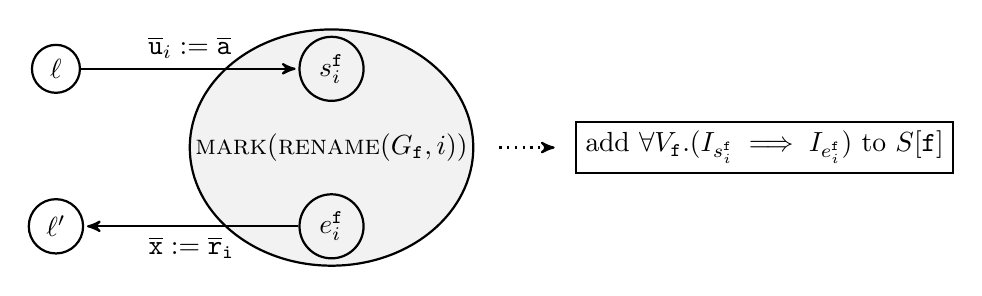
\begin{tikzpicture}[->,>=stealth',shorten >=1pt,auto,node
      distance=2cm,thick,node/.style={circle,draw}]

      \draw [fill=gray!10] (3.5, -1) ellipse (1.8 and 1.5);
      \node (text) at (3.5, -1) {$\textsc{mark}(\textsc{rename}(G_\fun{f},i))$};
      \node[node] (00) at (0, 0)  {$\ell$};
      \node[node] (01) at (0, -2) {$\ell'$};
      \node[node] (10) at (3.5, 0)  {$s_i^\fun{f}$};
      \node[node] (11) at (3.5, -2) {$e_i^\fun{f}$};

      \node (arrow_s) at (5.5, -1) {};
      \node (arrow_e) at (6.5, -1) {};
      
      \node[rectangle,text centered,draw] (text) at (9, -1)
      { add $\forall V_{\mathtt{f}}.
        (I_{s_i^\fun{f}} \implies I_{e_i^\fun{f}})$
        to $S[\fun{f}]$}; 
      
      \path
        (arrow_s) edge [dotted]
                  node {} (arrow_e)
        (00) edge 
             node {$\overline{\mathtt{u}}_i := \overline{\mathtt{a}}$} (10)

        (11) edge 
             node {$\overline{\mathtt{x}} := \mathtt{\overline{r}_i}$} (01) ;
    \end{tikzpicture}

  \caption{Updating Summary}
  \label{figure:updating-summary}
\end{figure}

\begin{proposition}
  \label{propposition:strengthen_postcondition}
  Given an unwound CFG $G^- = \langle V^-, E^-, \textmd{cmd}^-, \overline{\mathtt{u}}, \overline{\mathtt{r}},s,e \rangle$ and
  define $L'_\fun{f}=\{(s_i^\fun{f},e_i^\fun{f}):
  I_{s_i^\fun{f}} \mbox{ contains no return variable of }\fun{f} \wedge
  s_i^\fun{f}, e_i^\fun{f}\in E^-\}$.
  If $\assert{\mathtt{true}}\ \mathtt{\overline{r}} := \mathtt{f}
     (\overline{\mathtt{u}})\ \assert{S[\fun{f}]}$ holds, then
  $\assert{\mathtt{true}}\ \mathtt{\overline{r}} := \mathtt{f}
   (\overline{\mathtt{u}})\ \assert{(I_\ell \implies
     I_{\ell'})}$ for all $(\ell,\ell')\in L'_\mathtt{f}$.
\end{proposition}
The proposition holds because $S[\mathtt{f}]= \bigwedge_{(\ell,\ell')\in L'_\fun{f}}\forall V_\mathtt{f}. (I_\ell \implies I_{\ell'})$ implies $\forall V_\mathtt{f}. (I_\ell \implies I_{\ell'})$ for any pair $(\ell,\ell')\in L'_\fun{f}$, which implies $I_\ell \implies I_{\ell'}$ for the same pair of locations $(\ell,\ell')$.

\begin{proposition}
\label{propposition:invariant}
Given an unwound CFG $G^- = \langle V^-, E^-, \textmd{cmd}^-, \overline{\mathtt{u}}, \overline{\mathtt{r}},s,e \rangle$ and
  define $L'_\fun{f}=\{(s_i^\fun{f},e_i^\fun{f}):
  I_{s_i^\fun{f}} \mbox{ contains no return variable of }\fun{f} \wedge
  s_i^\fun{f}, e_i^\fun{f}\in E^-\}$.
We have $\assert{I_\ell}\
  \mathtt{\overline{r}} := \mathtt{f}
  (\overline{\mathtt{u}})\ \assert{I_\ell}$ for all $(\ell,\ell')\in L'_\mathtt{f}$
\end{proposition}
The proposition holds because $I_\ell$ is a formula over all variables in $G^-$ excepts $\mathtt{\overline{r}}$ and the only possible overlap with variables in $\mathtt{\overline{r}} := \mathtt{f} (\overline{\mathtt{u}})$ are the formal parameters $\overline{\mathtt{u}}$. However, we assume that values of formal parameters do not change in a function (see Section~\ref{section:preliminaries}), hence the values of all variables in $I_\ell$ will stay the same after the execution of the function call $\mathtt{\overline{r}} := \mathtt{f} (\overline{\mathtt{u}})$.


\subsection{Checking Summary}
\label{subsection:checking-summary}

Let $G_{\fun{f}} = \langle V, E, \textmd{cmd}, \overline{\mathtt{u}}, \overline{\mathtt{r}},s,e \rangle$ be the
control flow graph for the function $\fun{f}$ and $S[\bullet]$ an
array of function summaries. In order to check whether the function
summary $S[{\mathtt{f}}]$ for $\mathtt{f}$ specifies the relation 
between the formal parameters and return values of $\mathtt{f}$, 
we define another control flow graph
$\hat{G}_{\mathtt{f}}^S = \langle V, E, \hat{\textmd{cmd}}, \overline{\mathtt{u}}, \overline{\mathtt{r}},s,e \rangle$ where
\begin{equation*}
\hspace{-0.2cm}
  \begin{array}{rcl}
    \hat{\textmd{cmd}} (\ell, \ell') & = &
    \left\{
      \begin{array}{ll}
        \overline{\mathtt{x}} := 
        \overline{\mathtt{nondet}};
        \mathtt{assume\ S[{\mathtt{g}}]}[
        \mathtt{\overline{u}^g} \mapsto \overline{\mathtt{a}},
        \mathtt{\overline{r}^g} \mapsto \overline{\mathtt{x}}]    
        &
        \textmd{ if } \textmd{cmd} (\ell, \ell') = 
        \overline{\mathtt{x}} := \mathtt{g} (\overline{\mathtt{a}})\\
		\mathtt{\overline{r}} := \overline{\mathtt{e}}
        &
        \textmd{ if } \textmd{cmd} (\ell, \ell') = \mathtt{return\ }
        \overline{\mathtt{e}}\\
        \textmd{cmd} (\ell, \ell')
        &
		\textmd{ otherwise}        
      \end{array}
    \right.
  \end{array}
\end{equation*}
We use $\mathtt{\overline{u}^g}$ and $\mathtt{\overline{r}^g}$ to denote the formal parameters and return variables of the function $\fun{g}$.

\begin{figure}
  \centering
  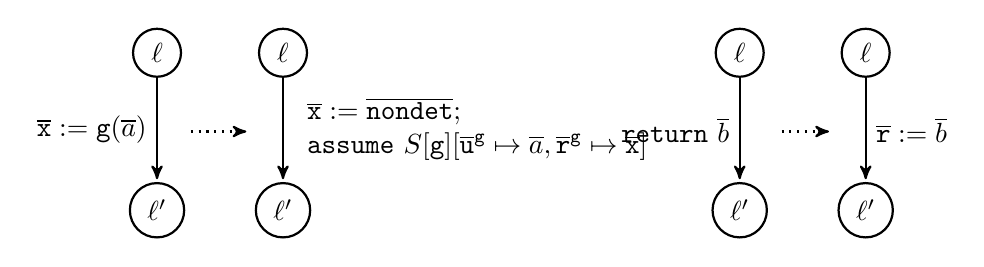
\begin{tikzpicture}[->,>=stealth',shorten >=1pt,auto,node
      distance=2cm,thick,node/.style={circle,draw}]

      \node[node] (00) at (0, 0)  {$\ell$};
      \node[node] (01) at (0, -2) {$\ell'$};

      \node (arrow_s0) at ( .3, -1) {};
      \node (arrow_e0) at (1.3, -1) {};

      \node[node] (10) at (1.6, 0)  {$\ell$};
      \node[node] (11) at (1.6, -2) {$\ell'$};

      \node[node] (20) at (7.4, 0)  {$\ell$};
      \node[node] (21) at (7.4, -2) {$\ell'$};

      \node (arrow_s1) at (7.8, -1) {};
      \node (arrow_e1) at (8.7, -1) {};

      \node[node] (30) at (9, 0)  {$\ell$};
      \node[node] (31) at (9, -2) {$\ell'$};

      
      \path
        (00) edge [left]
             node {$\overline{\mathtt{x}} := \mathtt{g}(\overline{a})$} (01)

        (arrow_s0) edge [dotted]
                  node {} (arrow_e0)

        (10) edge
             node {$
               \begin{array}{l}
                 \overline{\mathtt{x}} := \overline{\mathtt{nondet}};\\
                 \mathtt{assume\ }S[\mathtt{g}]
                 [\mathtt{\overline{u}^g} \mapsto \overline{a},
                  \mathtt{\overline{r}^g} \mapsto \overline{\mathtt{x}}]
               \end{array}
             $} (11)

        (20) edge [left]
             node {$\mathtt{return\ } \overline{b}$} (21) 

        (arrow_s1) edge [dotted]
                  node {} (arrow_e1)

        (30) edge 
             node {$\mathtt{\overline{r}} := \overline{b}$} (31) 
             ;
    \end{tikzpicture}

  \caption{Checking Summary}
  \label{figure:checking-summary}
\end{figure}

The control flow graph $\hat{G}_{\mathtt{f}}^S$ replaces every
function call in $G_{\mathtt{f}}$ by instantiating a function
summary. Using the proof rule for recursive functions, we have the
following proposition:
\begin{proposition}
  \label{proposition:check_summary}
  Let $G_{\fun{f}} = \langle V, E, \textmd{cmd}, \overline{\mathtt{u}}, \overline{\mathtt{r}},s,e \rangle$ be the control flow graph for the function
  $\mathtt{f}$, and $S[\bullet]$ an array of logic formulae over the formal
  parameters and return variables of each function. If $\assert{\top}\
  \hat{G}_{\mathtt{g}}^S\ \assert{S[\mathtt{g}]}$ for every
  function $\mathtt{g}$, then $\assert{\top}\ \mathtt{\overline{r}} :=
  \mathtt{f} (\overline{\mathtt{u}})\ \assert{S[\mathtt{f}]}$.
\end{proposition}

It is easy to check $\assert{\top}\ \hat{G}^S_{\mathtt{g}}\
\assert{S[\mathtt{g}]}$ by program analysis. Let $G_{\mathtt{f}}$ be
the control flow graph for the function $\mathtt{f}$ and
$\hat{G}^S_{\mathtt{f}} = \langle V, E, \hat{\textmd{cmd}}, \overline{\mathtt{u}}, \overline{\mathtt{r}},s,e \rangle$ as
above. Consider another control flow graph $\tilde{G}^S_{\mathtt{f}} =
\langle \tilde{V}, \tilde{E}, \tilde{\textmd{cmd}} , \overline{\mathtt{u}}, \overline{\mathtt{r}},s,e \rangle$ where
\begin{equation*}
  \begin{array}{rcl}
    \tilde{V} & = & V \cup \{ \tilde{\ell}_e \}\\
    \tilde{E} & = & E \cup \{ (\ell_e, \tilde{\ell}_e) \}\\
    \tilde{\textmd{cmd}} (\ell, \ell') & = &
    \left\{
      \begin{array}{ll}
        \hat{\textmd{cmd}} (\ell, \ell') & 
        \textmd{ if } (\ell, \ell') \in E\\
        \mathtt{assert\ } S[\mathtt{f}] &
        \textmd{ if } (\ell, \ell') = (\ell_e, \tilde{\ell}_e)
      \end{array}
    \right.
  \end{array}
\end{equation*}

\begin{corollary}
  Let $G_{\fun{f}} = \langle V, E, \textmd{cmd}, \overline{\mathtt{u}}, \overline{\mathtt{r}},s,e \rangle$ be the control flow graph for the function
  $\mathtt{f}$, and $S[\bullet]$ an array of logic formulae over the formal
  parameters and return variables of each function. If $\textsc{BasicChecker}
  (\tilde{G}^S_{\mathtt{g}})$ returns $\mathit{Pass}$ for every function
  $\mathtt{g}$, then $\assert{\top}\ \mathtt{\overline{r}} :=
  \mathtt{f} (\overline{\mathtt{u}})\ \assert{S[\mathtt{f}]}$.
  \label{corollary:check-summary}
\end{corollary}

\begin{algorithm}
  \KwIn{$G = \langle V, E, \textmd{cmd} \rangle$ : a control flow
    graph; $S[\bullet]$ : an array of function summaries}
  \KwOut{$\top$ if all function summaries are valid; $\bot$ otherwise}
  \ForEach{function $\mathtt{g}$}
  {
    \lIf{$\textsc{BasicChecker} (\tilde{G}^S_{\mathtt{g}}) \neq
      \mathit{Pass}$}
    {
      \Return $\bot$\;
    }
  }
  \Return $\top$\;
  \caption{$\textmd{CheckSummary} (G, S)$}
  \label{algorithm:check-summary}
\end{algorithm}
\subsection{Unwinding}
\label{subsection:unwinding}
We first define the rename function $\textsc{rename}(G)$. It returns a 5-tuple $(G^i, \bar{f}^i, \bar{r}^i,\ell_s^i,\ell_e^i)$ where $G^i$ is a CFG obtained by renaming all variables and locations in $G$ with a fresh index value $i$, $\bar{f}^i$ and $\bar{r}^i$ are formal parameters and return variables of $G^i$, and $\ell_s^i,\ell_e^i$ are the renamed entry and exit locations. The function $\textsc{unwind}(G)$ returns a CFG $G'$ obtained by replacing all function call edges in $G$ with the CFG of the called function after renaming. In order to help exacting summaries from the $G'$, $\textsc{unwind}(G)$ annotates in $G'$ the entry and exit locations ${\ell_s^i}$ and ${\ell_e^i}$ of the unwounded functions $f$ with superscript $(f)$, i.e., ${\ell_s^i}^{(f)}$ and ${\ell_e^i}^{(f)}$. The formal definition is given below.

Given a function $\mathtt{f}$ with CFG $G_f=\langle
V_f, E_f,\textmd{cmd}_f \rangle$.
Let $\hat{E} =\{e\in E: \textmd{cmd} (e)= (\bar{x}:=\mathtt{f}(\bar{a}))\}$ be the set of function call edges in $E$ and define a function $\textsc{toCFG}(e)$ that maps a call edge $e$ of function $f$ to a 5-tuple $\textsc{rename}(G_f)$. Notice that two different call edges of the same function are mapped to two different 5-tuples. If no location with superscript $(f)$ appear in $V$, $\textsc{toCFG}(e)$ returns a 5-tuple with entry and exit locations annotated with superscript $(f)$.

Formally, $\textsc{unwind}(G) = \langle V', E',\textmd{cmd}' \rangle$ such that (1) $V' = V\cup \bigcup\{V^i: e\in \hat{E} \wedge \textsc{toCFG}(e)= (\langle V^i, E^i,\textmd{cmd}^i \rangle, \bar{f}^i, \bar{r}^i,s,e) \}$ (2) $E'= E \setminus \hat{E} \cup \bigcup\{E_f\cup\{(\ell, s),(e, \ell')\}: (\ell, \ell')\in \hat{E} \wedge \textsc{toCFG}(\ell, \ell')= (\langle V^i, E^i,\textmd{cmd}^i \rangle, \bar{f}^i, \bar{r}^i,s,e) \}$ with $s\in \{\ell_s^i,{\ell_s^i}^{(f)}\}$, $e\in \{\ell_e^i,{\ell_e^i}^{(f)}\}$, $\textmd{cmd}' (\ell, {\ell_s^i}) = (\bar{a}=\bar{f})$, and $\textmd{cmd}' ({\ell_e^i}, \ell') = (\bar{x}=\bar{r})$.


%$\textsc{unwind}(G) = \langle
%V', E' \rangle$ such that 
%(1) For all edges $(\ell, \ell')\in E$ with $\textmd{cmd} (\ell, \ell')=$



\hide{
\begin{algorithm}
  \KwIn{$G = \langle V, E \rangle$ : a control flow graph}
  $V' \leftarrow V$\;
  $E' \leftarrow E$\;
  \ForEach{$(\ell, \ell')\in E$ with $\textmd{cmd} (\ell, \ell')= x_1,\ldots,x_n:=\mathtt{f}(E_1, \ldots, E_n)$}
  {
  	Let $G_f$ b
  
    \uIf {\textsc{BasicChecker} ($\underline{G}_k$) =
      $\mathit{ErrorTrace} (\tau)$}
    {
      \tcp{find an error trace in the under-approximation $\underline{G}_k$}
      \Return $\mathit{ErrorTrace} (\tau)$\;
    }
    \uElseIf {\textsc{BasicChecker} ($\overline{G}_k$) =
      $\mathit{Pass}$}
    {
      \tcp{prove all assertions in the over-approximation $\overline{G}_k$}
      \Return $\mathit{Pass}$\;
    }
    \uElse {
      $G_{k+1} \leftarrow $ unwind $G_k$\;
      $k \leftarrow k + 1$\;
    }
  }
  \caption{The $\textsc{unwind}(G)$ function}
  \label{algorithm:unwind}
\end{algorithm}
}

\begin{proposition}
  Let $G$ be a control flow graph, $P$ and $Q$ logic formulae with
  free variables over program variables of $G$. $\assert{P}\ G\ 
  \assert{Q}$ if and only if $\assert{P}\ \textsc{unwind} (G)\ \assert{Q}$.
\end{proposition}


\section{Experiments}
\label{section:experiments}

\newcommand{\safe}{S}
\newcommand{\unsafe}{U}
\newcommand{\unknown}{?}
\newcommand{\exception}{E}
\newcommand{\timeout}{T.O.}
\newcommand{\unknownmark}{\ensuremath{^?}}
\newcommand{\wrongmark}{\ensuremath{^!}}

\todo{parameters passed to these tools}

A prototype tool of our approach has been implemented with
\textsc{CPAChecker} as the underlying intraprocedure analyzer.
We compared our tool based on experiments with four participants,
namely Blast~\cite{BeyerHJM07}, CBMC~\cite{}, Ultimate
Automizer~\cite{HeizmannCDEHLNSP13}, and Ultimate Kojak~\cite{Kojak},
of the 2014 Competition on Software Verification (SV-COMP
2014)~\cite{svcomp14}.
The latter three tools are the top three winners of the
\textbf{recursive} category in the 2014 competition.
In our experiments, the programs under verification, including 16
bug-free and 7 buggy C programs, were selected from the
\textbf{recursive} category of SV-COMP 2014.
The experiments were performed on a virtual machine with one 2.93-GHz 
CPU and 4 GB of memory running 64-bit Ubuntu 12.04 LTS.
The virtual machine ran on a host with an Intel Core i7-870 Quad-Core
CPU and 8 GB of memory running 64-bit Windows 7.
The timeout of a verification task is 900 seconds.

The experimental results are summarized in
Table~\ref{table:experiments} where Iter. is \todo{?}, Time is
measured in seconds, the superscript $!$ or $?$ indicates that the
returned result is respectively incorrect or unknown, E indicates
exceptions, and T.O. indicates timeouts.
We use the score schema (shown in Table~\ref{table:score-schema}) in
SV-COMP 2014 to evaluate these tools.
Table~\ref{table:experiments} shows that our tool outperforms Ultimate
Automizer, Ultimate Kojak, and Blast in terms of scores.
Although CBMC got the highest score, several results returned by CBMC
may be doubtful because CBMC always reports safe if no bug is found
within a given set of bounds~\footnote{This was confirmed in a private
  communication with the developers of CBMC.}.
According to Table~\ref{table:experiments}, the bounds mighty be 850
seconds.
If we ignore results returned by CBMC exactly in 850 seconds, the gap
between the scores of CBMC and our tool becomes much smaller.

\begin{table}
\caption{Score schema.\label{table:score-schema}}
\begin{center}
\begin{tabular}{|c|c|c|}
\hline
Points & Program Correctness & Reported Result \\\hline
0      & TRUE or FALSE & UNKNOWN \\
+1     & FALSE         & FALSE \\
-4     & TRUE          & FALSE \\
+2     & TRUE          & TRUE \\
-8     & FALSE         & TRUE \\\hline
\end{tabular}
\end{center}
\end{table}

% ^*: the result is incorrect
% ^?: the result is unknown
\begin{table}
\caption{Experimental results of verifying programs in the
  \textbf{recursive} category of the 2014 Competition on Software
  Verification. The superscript $!$ or $?$ indicates that the
  returned result is respectively incorrect or unknown. E
  indicates exceptions while T.O. indicates
  timeouts.\label{table:experiments}}
\begin{tabular}{|c|cc|c|c|c|c|}
\hline
\multirow{2}{*}{Program} & \multicolumn{2}{c|}{Our Tool} &
Ultimate Automizer & Ultimate Kojak & CMBC-4.5 & Blast 2.7.2 \\ \cline{2-7}
& Iter. & Time  & Time  & Time  & Time  & Time \\ \hline
Ackermann01\_true.c      & 1 & 5.85                  & \timeout         & \timeout           & 850                   & \exception \\
Ackermann02\_false.c     & 4 & 54.625                & 4.151            & \timeout           & 1.036                 & \exception \\
Ackermann03\_true.c      &   & \timeout              & \timeout         & \timeout           & 850                   & \exception \\
Ackermann04\_true.c      &   & \timeout              & \timeout         & \timeout           & 850                   & \exception \\
Addition01\_true.c       & 2 & 13.71                 & \timeout         & \timeout           & 850                   & \exception \\
Addition02\_false.c      & 2 & 9.341                 & 3.745            & 3.523              & 0.26                  & 3.97 \\
Addition03\_false.c      &   & \timeout              & \timeout         & \timeout           & 850\wrongmark         & \exception \\
EvenOdd01\_true.c        &   & 2.763\wrongmark       & \timeout         & \timeout           & 1.293                 & 0.08\wrongmark \\
EvenOdd03\_false.c       &   & 2.757                 & 3.163            & 3.196              & 0.116                 & 0.08 \\
Fibonacci01\_true.c      & 6 & 300.045               & \timeout         & \timeout           & 850                   & \exception \\
Fibonacci02\_true.c      &   & \timeout              & 60.713           & 72.138\unknownmark & 0.834                 & \exception \\
Fibonacci03\_true.c      &   & \timeout              & \timeout         & \timeout           & 850                   & \exception \\
Fibonacci04\_false.c     & 5 & 103.496               & 7.438            & 8.155              & 0.409                 & \exception \\
Fibonacci05\_false.c     &   & \timeout              & 128.911          & 23.174             & 557.18                & \exception \\
gcd01\_true.c            & 1 & 5.843                 & 5.369            & 7.26               & 850                   & 16.074\wrongmark \\
gcd02\_true.c            &   & \exception            & \timeout         & \timeout           & 850                   & \exception \\
McCarthy91\_false.c      & 1 & 7.255                 & 3.152            & 3.09               & 0.258                 & 0.086 \\
McCarthy91\_true.c       & 2 & 11.982                & 81.32            & 6.783              & 850                   & 16.237\wrongmark \\
MultCommutative\_true.c  &   & \exception            & \timeout         & \timeout           & 850                   & \exception \\
Primes\_true.c           &   & \exception            & \timeout         & \timeout           & 850                   & \exception \\
recHanoi01\_true.c       &   & \timeout              & \timeout         & \timeout           & 850                   & \exception \\
recHanoi02\_true.c       & 1 & 5.172                 & \timeout         & \timeout           & 0.749                 & 1.897\wrongmark \\
recHanoi03\_true.c*      &   & \exception            & \timeout         & \timeout           & 0.713                 & \exception \\
\hline\hline
correct results          & \multicolumn{2}{c|}{11}   & 9                & 7                  & 22 (10)               & 3 \\ 
false negative           & \multicolumn{2}{c|}{0}    & 0                & 0                  & 1 (0)                 & 0 \\
false positive           & \multicolumn{2}{c|}{1}    & 0                & 0                  & 0 (0)                 & 4 \\
score                    & \multicolumn{2}{c|}{13}   & 12               & 9                  & 30 (14)               & -13 \\
\hline
\end{tabular}
\end{table}

%%% Local Variables: 
%%% mode: latex
%%% TeX-master: "draft"
%%% LaTeX-command: "latex -shell-escape"
%%% End: 


\section{Discussion}
\label{section:conclusion}
% Extension: using program analyzer + bounded model checking

The number of unwindings is perhaps the most important factor in our
recursive analysis technique (Table~\ref{table:experiments}). We find
that \textsc{CPAChecker} performs poorly when many unwindings are
needed. We however do not enable the more efficient block encoding in
\textsc{CPAChecker} for the ease of implementation. One can improve
the performance of our algorithm with the efficient but complicated
block encoding. A bounded analyzer may also speed up the
verification of bounded properties. 

Our algorithm extracts function summaries from inductive invariants. 
There are certainly many heuristics to optimize the computation of
function summaries. For instance, some program analyzers return error
traces when properties fail. Particularly, a valuation of formal
parameters is obtained when \textmd{CheckSummary}
(Algorithm~\ref{algorithm:check-summary}) returns $\FF$. If the
valuation is not possible in the $\mathtt{main}$ function, one can use
its inductive invariant to refine function summaries. We in 
fact exploit error traces computed by \textsc{CPAChecker} in the
implementation. 
\hide{
\noindent
\textbf{Related Works.}
In~\cite{LalR08,LalR09}, a reduction technique for checking context-bounded concurrent programs to sequential analysis is developed. Numerous intraprocedural analysis techniques have been developed over the years. Many tools are in fact freely available (see, for instance, \textsc{Blast}~\cite{BeyerHJM07}, \textsc{CPAChecker}~\cite{BeyerK11}, and \textsc{UFO}~\cite{AlbarghouthiLGC12}). Interprocedural analysis techniques are also available (see~\cite{RepsHS95,BallR01,CousotCFMMMR05,CuoqKKPSY12,coverity,polyspace} for a hopelessly incomplete list). Recently, recursive analysis attracts new attention. The Competition on Software Verification adds a new category for recursive programs in 2014~\cite{svcomp14}. Among the participants, \textsc{CBMC}~\cite{ClarkeKL04}, \textsc{Ultimate Automizer}~\cite{HeizmannCDEHLNSP13}, and \textsc{Ultimiate Kojak}~\cite{Kojak} are the top three tools for the recursive category. Our work is inspired by \textsc{Whale}~\cite{AlbarghouthiGC12}. Similar to \textsc{Whale}, we apply a Hoare logic proof rule for recursive calls. However, our technique works on control flow graphs and builds on an intraprocedural analysis tool. It is hence very lightweight and modular. Better intraprocedural analysis tools easily give better recursive analysis through our technique. \textsc{Whale}, on the other hand, analyzes by exploring abstract reachability graphs. Since \textsc{Whale} extends summary computation and covering relations for recursion, its implementation is more involved. Although \textsc{Whale} is able to analyze recursive program in theory, its implementation does not appear to support this feature.}


\bibliographystyle{plain}
\bibliography{refs}

\end{document}